%!TEX root = ../../main.tex

\begin{frame}[plain]
	\section{Satz 1: Zweifärbbarkeit von Hypergraphen}
\end{frame}

\begin{frame}{Hypergraphen}
	\begin{definition}[$k$-uniformer Hypergraph]
		\vspace{0.25cm}
		Ein $k$-uniformer Hypergraph $\mathcal{H}$ ist ein geordnetes Paar $(V; E)$, wobei $V$ die Menge der Knoten und $E = \{e_1, e_2, ..., e_n\} \subseteq \binom{V}{k}$ die Menge der Hyperkanten ist ($k$-Tupel der Knoten). \cite{Matousek2008}
	\end{definition}
	
	\onslide<2->{
		\begin{itemize}
			\item $E \subseteq \{e \in \mathcal{P}(V) \: | |e|=k\}$
			\item \enquote{gewöhnlicher} Graph: Hypergraph mit $k=2$
		\end{itemize}
	}
\end{frame}

\begin{frame}{Hypergraphen}
	\begin{figure}
		\includegraphics[width=\linewidth]{content/fig/1-hypergraph3}
		\caption{Hypergraph mit $k=3$\footnote{https://www.researchgate.net/figure/Correspondence-between-a-mathematical-3-uniform-hypergraph-and-the-quantum-state\_fig5\_233753189}}
	\end{figure}
\end{frame}

\begin{frame}{Färbbarkeit von Hypergraphen}
	\begin{definition}[$c$-Färbbarkeit von Hypergraphen]
		\vspace{0.25cm}
		Ein Hypergraph $\mathcal{H}$ ist $c$-färbbar, wenn seine Knoten mit $c$ Farben gefärbt werden können, sodass keine Kante von $\mathcal{H}$ monochrom ist. \cite{Matousek2008}
	\end{definition}
	
	\onslide<2->{
		\begin{itemize}
			\item keine Kante besitzt nur Knoten einer Farbe (für $c>1$)
		\end{itemize}
	}
	
	\onslide<3->{
		\vspace{0.5cm}	
		\begin{framed}
			Was ist die kleinste Anzahl an Kanten, ab welcher ein Hypergraph $\mathcal{H}$ existieren kann, welcher nicht mehr $2$-färbbar ist?
    	\end{framed}
	}
\end{frame}

\begin{frame}{$2$-Färbbarkeit von Hypergraphen}
	\begin{definition}[$m(k)$]
		\vspace{0.25cm}
		Sei \textbf{$m(k)$} die kleinste Anzahl an Kanten in einem $k$-uniformen Hypergraphen $\mathcal{H}$, für welchen eine Konfiguration existiert, welche nicht valide 2-färbbar ist. \cite{Matousek2008}
	\end{definition}
	
	\onslide<2->{
		\begin{itemize}
			\item \textbf{nicht}: Es existiert kein $\mathcal{H}$ mit $|E|\geq m(k)$, welches eine valide $2$-Färbung hat.
			\item \textbf{eher}: Es existiert (mind.) ein $\mathcal{H}$  mit $|E| \geq m(k)$, welches \textbf{keine} valide $2$-Färbung hat.
			\item \textbf{aber}: alle $\mathcal{H}$ mit $|E| < m(k)$ haben eine valide $2$-Färbung.
		\end{itemize}
	}
\end{frame}

\begin{frame}{$2$-Färbbarkeit von Hypergraphen}
	\begin{figure}
		\onslide<1->{
			\subcaptionbox{$K_3$}[0.3\linewidth]{
				\only<1,5->{
					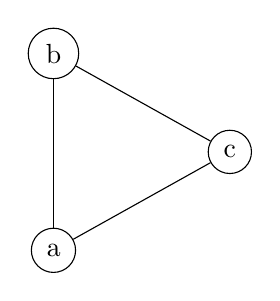
\begin{tikzpicture}
						\node (a) at (0,0) [draw=black,circle] {a};
						\node (b) at (0,2.5) [draw=black,circle] {b};
						\node (c) at (2.24,1.25) [draw=black,circle] {c};
						\draw (b) -- (c);
						\draw (a) -- (b);
						\draw (a) -- (c);
					\end{tikzpicture}
				}%
				\only<2>{
					\begin{tikzpicture}
						\node (a) at (0,0) [draw=mLightBrown,circle] {a};
						\node (b) at (0,2.5) [draw=mLightGreen,circle] {b};
						\node (c) at (2.24,1.25) [draw=mLightGreen,circle] {c};
						\draw [mLightGreen,] (b) -- (c);
						\draw (a) -- (b);
						\draw (a) -- (c);
					\end{tikzpicture}
				}%
				\only<3>{
					\begin{tikzpicture}
						\node (a) at (0,0) [draw=mLightGreen,circle] {a};
						\node (b) at (0,2.5) [draw=mLightBrown,circle] {b};
						\node (c) at (2.24,1.25) [draw=mLightGreen,circle] {c};
						\draw (b) -- (c);
						\draw (a) -- (b);
						\draw [mLightGreen,] (a) -- (c);
					\end{tikzpicture}
				}%
				\only<4>{
					\begin{tikzpicture}
						\node (a) at (0,0) [draw=mLightGreen,circle] {a};
						\node (b) at (0,2.5) [draw=mLightGreen,circle] {b};
						\node (c) at (2.24,1.25) [draw=mLightBrown,circle] {c};
						\draw (b) -- (c);
						\draw [mLightGreen,] (a) -- (b);
						\draw (a) -- (c);
					\end{tikzpicture}
				}%
			}
		}
		\onslide<5->{
			\subcaptionbox{Quadrat $ABCD$}[0.3\linewidth]{
				\begin{tikzpicture}
					\only<5,7->{
						\node (a) at (0,0) [draw=black,circle] {a};
						\node (b) at (0,2.5) [draw=black,circle] {b};
						\node (c) at (2.5,2.5) [draw=black,circle] {c};
						\node (d) at (2.5,0) [draw=black,circle] {d};
					}
					\only<6>{
						\node (a) at (0,0) [draw=mLightGreen,circle] {a};
						\node (b) at (0,2.5) [draw=mLightBrown,circle] {b};
						\node (c) at (2.5,2.5) [draw=mLightGreen,circle] {c};
						\node (d) at (2.5,0) [draw=mLightBrown,circle] {d};
					}
					\only<5->{
						\draw (a) -- (b);
						\draw (a) -- (d);
						\draw (b) -- (c);
						\draw (c) -- (d);
					}
				\end{tikzpicture}
			}
		}
		\onslide<7->{
			\subcaptionbox{\textsc{Faro}-Konfiguration}[0.3\linewidth]{
				\begin{tikzpicture}
					\node (a) at (0,0) [draw=black,circle,fill=bg] {a};
					\draw [mLightGreen,]( 0,0) circle (.75cm);
					\node (e) at (90:1.5cm) [draw=black,circle] {e};
					\node (f) at (210:1.5cm) [draw=black,circle] {f};
					\node (g) at (330:1.5cm) [draw=black,circle] {g};
					\node (b) at (150:.75cm) [draw=black,circle,fill=bg] {b};
					\node (c) at (270:.75cm) [draw=black,circle,fill=bg] {c};
					\node (d) at (30:.75cm) [draw=black,circle,fill=bg] {d};
					\draw [blue,] (e) -- (b) -- (f);
					\draw [red,] (f) -- (c) -- (g);
					\draw [mLightBrown,] (g) -- (d) -- (e);
					\draw [purple,] (b) -- (a) -- (g);
					\draw [gray,] (d) -- (a) -- (f);
					\draw [] (c) -- (a) -- (e);
				\end{tikzpicture}
			}
		}
		\caption{Beispiele für Kantenfärbung}
	\end{figure}

	\begin{itemize}
		\item<1-> für $k=2 \rightarrow m(2)=3$: $K_3$ (\textit{Beweis.} Trivial.)
		\item<7-> für $k=3 \rightarrow m(3)=7$: \textsc{Faro}-Konfiguration (\textit{Beweis.} Sehr komplex.)
		\item<8-> für $k>4 \rightarrow m(k)$ unbekannt, untere Schranke jedoch vorhanden.
	\end{itemize}
\end{frame}

\begin{frame}{$2$-Färbbarkeit von Hypergraphen}

	\begin{framed}
		\begin{satz}
			\vspace{0.25cm}
			Jeder Hypergraph $\mathcal{H}$ mit höchstens $2^{k-1}$ Kanten ist (gerade so) 2-färbbar. Es gilt 
			\begin{equation*}
				m(k) > 2^{k-1}
			\end{equation*}
		\end{satz}
	\end{framed}
	
	\onslide<2->{
		\vspace{0.25cm}
		\textit{Beweis.} Mithilfe der probabilistischen Methode zeigen wir, dass alle $\mathcal{H}$ mit $|E|\leq 2^{k-1}$ valide $2$-färbbar sind und betrachten dann den Gegenfall.
	}
	
	\onslide<3->{\qed}
	
\end{frame}

